\documentclass[a4paper, 12pt]{article}
\usepackage[utf8]{inputenc}
\usepackage{amsmath,amsfonts,amsthm,amssymb,longtable,listings,graphicx, float, epstopdf, textcomp}
\usepackage{mathtools}
\usepackage[finnish]{babel}
\usepackage{tikz}
\usetikzlibrary{positioning}
\renewcommand{\contentsname}{Sisällysluettelo}
\renewcommand{\abstractname}{Abstrakti}
\theoremstyle{definition}
\newtheorem{mydef}{Määritelmä}
\newtheorem{huom}{Huomautus}
\newtheorem{lemma}{Lemma}
\newtheorem{example}[mydef]{Esimerkki}
\theoremstyle{plain}
\newtheorem{teor}[mydef]{Lause}


\lstset{basicstyle=\small, frame=single}

\begin{document}

\title{Graafien automorfismiryhmä}
\author{Juuso Valli}
\date{24. 9. 2017}

\maketitle

\begin{abstract}
% TBW
\end{abstract}

\tableofcontents

\newpage

\section{Määritelmiä ja merkintöjä}

Olkoon $V$ äärellinen joukko. Olkoon $E(V) = \{\{u, v\} | u, v \in V, u \neq v\}$ joukon $V$ alijoukkojen joukko, jonka jäsenet sisältävät täsmälleen kaksi eri solmua.
Olkoon \emph{graafi} $G = (V, E), E \subseteq E(V)$. Joukkoa $V$ kutsutaan graafin $G$ \emph{solmuiksi}, ja joukkoa $E$ kutsutaan \emph{kaariksi}. Annetun graafin solmujoukosta kätetään merkintää $G_V$, ja kaarijoukosta merkintää $G_E$.
Kaaresta $\{u, v\}$ käytetään merkintää $uv$. Huomaa että näillä merkinnöillä $uv = vu$.
Yksinkertaisuuden vuoksi solmuista käytetään myös merkintää $v \in G$ merkinnän $v \in G_V$ sijaan.

Olkoon $G$ ja $H$ graafeja. Graafit $G$ ja $H$ ovat \emph{isomorfiset} $G \cong H$ mikäli on olemassa bijektio $f: V_G \rightarrow V_H$ siten, että
\begin{center}
\begin{math}
uv \in E_G \Longleftrightarrow f(u)f(v) \in E_H
\end{math}
\end{center}
kaikilla $u, v \in G$.

Tällaisia bijektioita kutsutaan \emph{isomorfismeiksi}.

Graafin $G$ \emph{automorfismit} ovat sen isomorfismeja itsensä kanssa. Triviaalisti nähdään että identiteettikuvaus on kaikkien graafien automorfismi, mutta graafeilla voi olla myös muita automorfismeja.

\begin{example}
\label{ex:d4}
Olkoon graafi $G = (\{v_1, v_2, v_3, v_4\}, \{v_1v_2, v_2v_3, v_3v_4, v_4v_1\})$.

\begin{center}
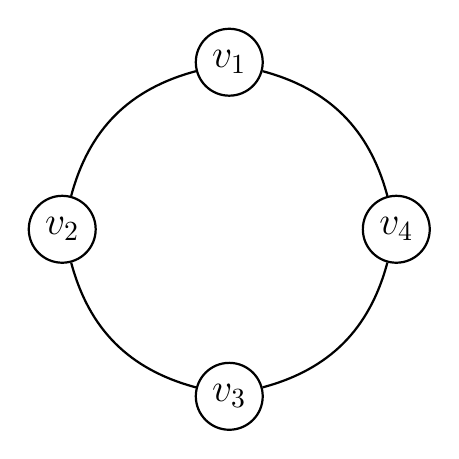
\begin{tikzpicture} [auto, node distance=3cm, every loop/.style={},
                    thick,solmu/.style={circle,draw,font=\sffamily\Large\bfseries}]

\node[solmu] (1) {$v_1$};
\node[solmu] (2) [below left of=1] {$v_2$};
\node[solmu] (3) [below right of=2] {$v_3$};
\node[solmu] (4) [below right of=1] {$v_4$};

 \path[every node/.style={font=\sffamily\small}]
    (1) edge [bend right] node[left] {} (2)
    (2) edge [bend right] node[left] {} (3)
    (3) edge [bend right] node[right] {} (4)
    (4) edge [bend right] node[right] {} (1);
\end{tikzpicture}
\end{center}

Olkoon kuvaus $f: V_G \rightarrow V_G, f(v_1) = v_2, f(v_2) = v_3, f(v_3) = v_4, f(v_4) = v_1$. Kuvaus $f$ on selvästi bijektio. Se, että kuvaus $f$ on automorfismi voidaan tarkistaa suoraan määritelmästä.

\begin{center}
\begin{tabular} {l l l}
$G_E$ & $f(u)f(v)$ & $f^{-1}(u)f^{-1}(v)$ \\
\hline
$v_1v_2$ & $ v_2v_3$ & $v_4v_1$ \\
$v_2v_3$ & $ v_3v_4$ & $v_1v_2$ \\
$v_3v_4$ & $v_4v_1$ & $v_2v_3$ \\
$v_4v_1$ & $v_1v_2$ &  $v_3v_4$ \\
\end{tabular}

\end{center}
\end{example}

\section{Automorfismiryhmä}

Olkoon $G_S$ graafin $G$ automorfismien joukko.

\begin{lemma}
\label{lemma:binaarirelaatio}
Kuvausten kompositio on binäärirelaatio $\circ : G_S \times G_S \rightarrow G_S$.
\begin{proof}
Olkoon $u, v \in G$. Olkoon $f, g \in G_S$.
\begin{center}
\begin{math}
uv \in E_G \xLeftrightarrow{g \in G_S} g(u)g(v) \in E_G  \xLeftrightarrow{f \in G_S} f(g(u))f(g(v)) \in E_G 
\end{math}
\end{center}
joten $f \circ g \in G_S$.
\end{proof}
\end{lemma}

\begin{lemma}
\label{lemma:identiteetti}
Jokaisella graafilla on identiteettikuvaus, joka on automorfismi.
\begin{proof}
Olkoon $u, v \in G$. Olkoon $id: G_V \rightarrow G_V, id(x) = x \forall x \in G_V$.
\begin{center}
\begin{math}
uv \in E_G \xLeftrightarrow{id(x) = x} id(u)id(v) \in E_G  
\end{math}
\end{center}
joten $id \in G_S$.
\end{proof}
\end{lemma}

\begin{lemma}
\label{lemma:kaanteiskuvaus}
Automorfismin $f$ käänteiskuvaus $f^{-1}$ on automorfismi.
\begin{proof}
Olkoon $u, v \in G$.
\begin{center}
\begin{math}
f^{-1}(u)f^{-1}(v) \in E_G \xLeftrightarrow{f \in G_S} f(f^{-1}(u))f(f^{-1}(v)) \in E_G \Leftrightarrow uv \in E_G
\end{math}
\end{center}
joten $f^{-1} \in G_S$.
\end{proof}
\end{lemma}

\begin{teor}
Pari $(G_S, \circ)$ on ryhmä.
\begin{proof}
Lemman \ref{lemma:binaarirelaatio} mukaan $\circ$ on $G_S$:n binäärirelaatio. Assosiatiivisuus on selvä kuvausten komposition assosiatiivisuuden perusteella. Lemman \ref{lemma:identiteetti} mukaan jokainen $G_S$ sisältää identiteettikuvauksen $id$, joka on ryhmän neutraalialkio. Lemman \ref{lemma:kaanteiskuvaus} mukaan jokaisella automorfismilla $f$ on vasta-alkio $f^{-1} \in G_S$ siten, että $f \circ f^{-1} = id$.
\begin{center}
\begin{math}
\end{math}
\end{center}
\end{proof}
\end{teor}

Graafin automorfismiryhmää kutsutaan myös graafin symmetriaryhmäksi.

\begin{huom}
Graafien automorfismiryhmät eivät yleisesti ole kommutatiivisia.\\
Tämä nähdään helposti vastaesimerkin kautta. Tarkastellaan esimerkin \ref{ex:d4} mukaista graafia. Olkoon $f$ esimerkissä esitetty automorfismi. Olkoon kuvaus $g: V_G \rightarrow V_G, g(v_1) = v_1, g(v_2) = v_4, g(v_3) = v_3, g(v_4) = v_2$. Kuvaus $g$ on selvästi myös graafin $G$ automorfismi. Mikäli automorfismiryhmä olisi kommutatiiviinen, olisi $f \circ g = g \circ f$. Kirjoittamalla kuvaukset auki nähdään että $f \circ g(v_1) = f(g(v_1)) = f(v_1) = v_2$, mutta toisaalta $g \circ f (v_1) = g(f(v_1)) = g(v_2) = v_4$, mistä seuraa ristiriita.
\end{huom}

\begin{example}
Esimerkin \ref{ex:d4} mukaisen graafin symmetriaryhmä $G_S$ on isomorfinen diedriryhmän $D_4$ kanssa. Yleisemmin $n$:n alkion rengasgraafi on isomorfinen diedriryhmän $D_n$ kanssa. Tämä nähdään helposti tarkastelemalla $G_S$:n ryhmätaulua. Otetaan $G_S$:n alkioille käyttöön seuraavat merkinnät: $\alpha_{i, j} \in G_S, 0 <0 i \leq n, j \in \{0, 1\}$ , siten että $\alpha_{i, j}$ kuvaa alkion $v_1$ alkioksi $v_i$ ja kääntää rengasgraafin suunnan mikäli $j = 1$. Tällä tavoin määriteltyjen isomorfismien lisäksi $G_S$:llä ei ole muita isomorfismeja.

Näitä merkintöjä käyttäen $G_S$:n symmeriaryhmän ryhmätaulu on seuraavanlainen tapauksessa $n=4$:

\begin{center}
\begin{tabular} {l | l l l l l l l l}
	                & $\alpha_{1, 0}$ & $\alpha_{2, 0}$ & $\alpha_{3, 0}$ & $\alpha_{4, 0}$ & $\alpha_{1, 1}$ & $\alpha_{2, 1}$ & $\alpha_{3, 1}$ & $\alpha_{4, 1}$ \\
\hline
$\alpha_{1, 0}$ & $\alpha_{1, 0}$ & $\alpha_{2, 0}$ & $\alpha_{3, 0}$ & $\alpha_{4, 0}$ & $\alpha_{1, 1}$ & $\alpha_{2, 1}$ & $\alpha_{3, 1}$ & $\alpha_{4, 1}$ \\
$\alpha_{2, 0}$ & $\alpha_{2, 0}$ & $\alpha_{3, 0}$ & $\alpha_{4, 0}$ & $\alpha_{1, 0}$ & $\alpha_{2, 1}$ & $\alpha_{3, 1}$ & $\alpha_{4, 1}$ & $\alpha_{1, 1}$ \\
$\alpha_{3, 0}$ & $\alpha_{3, 0}$ & $\alpha_{4, 0}$ & $\alpha_{1, 0}$ & $\alpha_{2, 0}$ & $\alpha_{3, 1}$ & $\alpha_{4, 1}$ & $\alpha_{1, 1}$ & $\alpha_{2, 1}$ \\
$\alpha_{4, 0}$ & $\alpha_{4, 0}$ & $\alpha_{1, 0}$ & $\alpha_{2, 0}$ & $\alpha_{3, 0}$ & $\alpha_{4, 1}$ & $\alpha_{1, 1}$ & $\alpha_{2, 1}$ & $\alpha_{3, 1}$ \\
$\alpha_{1, 1}$ & $\alpha_{1, 1}$ & $\alpha_{4, 1}$ & $\alpha_{3, 1}$ & $\alpha_{2, 1}$ & $\alpha_{1, 0}$ & $\alpha_{4, 0}$ & $\alpha_{3, 0}$ & $\alpha_{2, 0}$ \\
$\alpha_{2, 1}$ & $\alpha_{2, 1}$ & $\alpha_{1, 1}$ & $\alpha_{4, 1}$ & $\alpha_{1, 1}$ & $\alpha_{2, 0}$ & $\alpha_{1, 0}$ & $\alpha_{4, 0}$ & $\alpha_{1, 0}$ \\
$\alpha_{3, 1}$ & $\alpha_{3, 1}$ & $\alpha_{2, 1}$ & $\alpha_{1, 1}$ & $\alpha_{4, 1}$ & $\alpha_{3, 0}$ & $\alpha_{2, 0}$ & $\alpha_{1, 0}$ & $\alpha_{4, 0}$ \\
$\alpha_{4, 1}$ & $\alpha_{4, 1}$ & $\alpha_{3, 1}$ & $\alpha_{2, 1}$ & $\alpha_{3, 1}$ & $\alpha_{4, 0}$ & $\alpha_{3, 0}$ & $\alpha_{2, 0}$ & $\alpha_{3, 0}$ \\
\end{tabular}
\end{center}


\end{example}

\begin{example}
Suoran graafin symmetriaryhmä on $C_2$.

\begin{center}
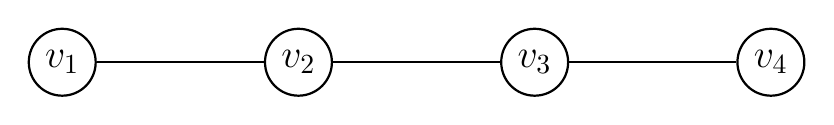
\begin{tikzpicture} [auto, node distance=3cm, every loop/.style={},
                    thick,solmu/.style={circle,draw,font=\sffamily\Large\bfseries}]

\node[solmu] (1) {$v_1$};
\node[solmu] (2) [right of=1] {$v_2$};
\node[solmu] (3) [right of=2] {$v_3$};
\node[solmu] (4) [right of=3] {$v_4$};

 \path[every node/.style={font=\sffamily\small}]
    (1) edge node[left] {} (2)
    (2) edge node[left] {} (3)
    (3) edge node[left] {} (4);
\end{tikzpicture}
\end{center}

Suoran graafin päädyissä olevilla alkioiden aste on $1$, ja kaikkien muiden alkoiden aste on $2$. Tästä seuraa se, että graafin päätyalkioit voidaan kuvata vain päätyalkoihin, sillä isomorfismit säilyttävät alkioiden asteen. Yhden päätyalkion kuvan määrääminen riittää määräämään koko graafin kuvan, joten mahdollisia kuvauksia on vain kaksi: $id$ ja kuvaus $f$, joka vaihtaa päätyalkioit keskenään. Koska $f \circ f = id$, graafin automorfismiryhmä on $C_2$
\end{example}

\begin{example}
Täyden graafin $K_n$ symmetriaryhmä on $S_n$.

\begin{center}
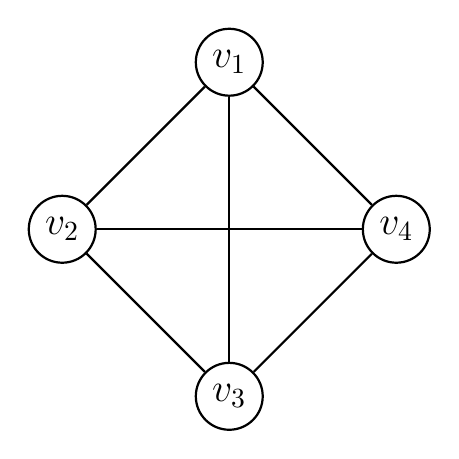
\begin{tikzpicture} [auto, node distance=3cm, every loop/.style={},
                    thick,solmu/.style={circle,draw,font=\sffamily\Large\bfseries}]

\node[solmu] (1) {$v_1$};
\node[solmu] (2) [below left of=1] {$v_2$};
\node[solmu] (3) [below right of=2] {$v_3$};
\node[solmu] (4) [below right of=1] {$v_4$};

 \path[every node/.style={font=\sffamily\small}]
    (1) edge node[left] {} (2)
    (1) edge node[left] {} (3)
    (1) edge node[left] {} (4)
    (2) edge node[left] {} (3)
    (2) edge node[left] {} (4)
    (3) edge node[left] {} (4);
\end{tikzpicture}
\end{center}

Koska jokainen alkio on kaikkien muiden alkioiden naapuri, jokainen $K_n$:n bijektio itsensä kanssa on automorfismi. Tästä seuraa se, että $K_n$:n automorfismiryhmä on $\Sigma(K_n) \simeq S_n$.
\end{example}

\begin{example}
Täysin kaksijakoisen graafin $K_{nm}, n \neq m$ symmetriaryhmä on $S_n \times S_m$.

\begin{center}
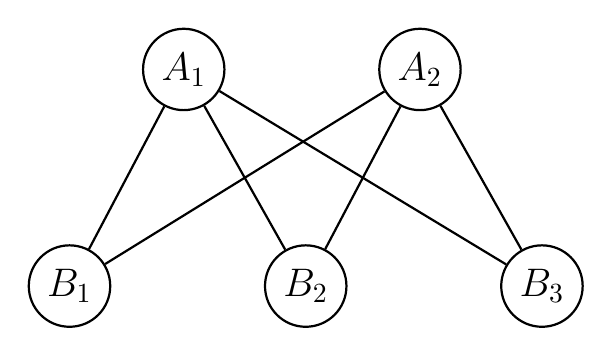
\begin{tikzpicture} [auto, node distance=3cm, every loop/.style={},
                    thick,solmu/.style={circle,draw,font=\sffamily\Large\bfseries}]

\node[solmu] (1) {$A_1$};
\node[solmu] (2) [right of=1] {$A_2$};
\node[solmu] (3) [below left=2cm and 0.7cm  of 1] {$B_1$};
\node[solmu] (4) [right of=3] {$B_2$};
\node[solmu] (5) [right of=4] {$B_3$};

 \path[every node/.style={font=\sffamily\small}]
    (1) edge node[left] {} (3)
    (1) edge node[left] {} (4)
    (1) edge node[left] {} (5)
    (2) edge node[left] {} (3)
    (2) edge node[left] {} (4)
    (2) edge node[left] {} (5);
\end{tikzpicture}
\end{center}

Olkoon $A, B \subset G_v$ graafin ylä- ja alakomponenit. Olkoon $H = \{f \in G_S : f|_B = id\}, K = \{f \in G_S : f|_A = id\}$. Kumpikin osajoukko on selvästi aliryhmä, sillä $(f \circ g)|_X = id$ jos $f|_X = id, g|_X = id$. Lisäksi nähdään että $H \cap K = \{ id \}$.

Määritellään funktion jako seuraavasti:

\begin{center}
\begin{math}
f_X(x) =
\left\{
	\begin{array}{ll}
		f(x)  & \mbox{jos } x \in X \\
		x & \mbox{jos } x \notin X
	\end{array}
\right.
\end{math}
\end{center}

Mielivaltainen automorfismi $f$ voidaan jakaa kahteen osaan joukkojen $A$ ja $B$ mukaan, josta saadaan $f = f_A \circ f_B, f_A \in K, f_B \in H$. Tästä seuraa että $G = HK$.

Olkoon $h \in H, k \in K$. Olkoon $x \in A$. 
\begin{center}
\begin{math}
(h \circ k)(x) = (id \circ k)(x) = (k \circ id)(x) = (k \circ h)(x)
\end{math}
\end{center}
Toisaalta jos $x \in B$:
\begin{center}
\begin{math}
(h \circ k)(x) = (h \circ id)(x) = (id \circ h)(x) = (k \circ h)(x)
\end{math}
\end{center}

Eli $hk = kh$. Tästä seuraa että $G_S = H \times K$.
\end{example}

\begin{example}
Täysin kaksijakoisen graafin $K_{nn}$ symmetriaryhmä on $C_2 \rtimes S_n^2$.

\begin{center}
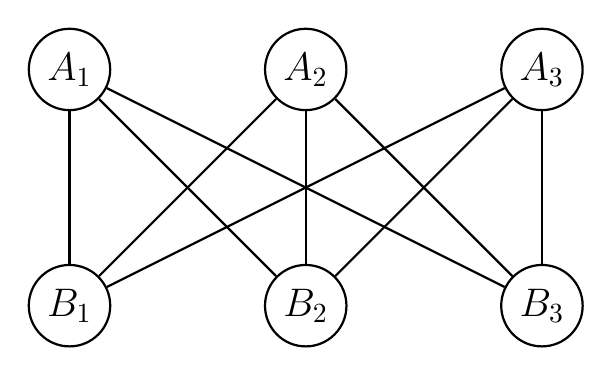
\begin{tikzpicture} [auto, node distance=3cm, every loop/.style={},
                    thick,solmu/.style={circle,draw,font=\sffamily\Large\bfseries}]

\node[solmu] (1) {$A_1$};
\node[solmu] (2) [right of=1] {$A_2$};
\node[solmu] (3) [right of=2] {$A_3$};
\node[solmu] (4) [below of=1] {$B_1$};
\node[solmu] (5) [right of=4] {$B_2$};
\node[solmu] (6) [right of=5] {$B_3$};

 \path[every node/.style={font=\sffamily\small}]
    (1) edge node[left] {} (4)
    (1) edge node[left] {} (5)
    (1) edge node[left] {} (6)
    (2) edge node[left] {} (4)
    (2) edge node[left] {} (5)
    (2) edge node[left] {} (6)
    (3) edge node[left] {} (4)
    (3) edge node[left] {} (5)
    (3) edge node[left] {} (6);
\end{tikzpicture}
\end{center}

Olkoon $A, B \subset G_v$ graafin ylä- ja alakomponenit, ja olkoon kummassakin komponentissa indeksointi lukujen $1 \dots n$ yli. Tarkastellaan automorfismiryhmän aliryhmää $H = \{f \in G_S : f(A) = A\}$
Olkoon $A, B \subset G_v$ graafin vasen ja oikea puoli. Olkoon $H = \{f \in G_S : f|_B = id\}, K = \{f \in G_S : f|_A = id\}$. Kumpikin osajoukko on selvästi aliryhmä, sillä $(f \circ g)|_X = id$ jos $f|_X = id, g|_X = id$. Lisäksi nähdään että $H \cap K = \{ id \}$.

Määritellään funktion jako seuraavasti:

\begin{center}
\begin{math}
f_X(x) =
\left\{
	\begin{array}{ll}
		f(x)  & \mbox{jos } x \in X \\
		x & \mbox{jos } x \notin X
	\end{array}
\right.
\end{math}
\end{center}

Mielivaltainen automorfismi $f$ voidaan jakaa kahteen osaan joukkojen $A$ ja $B$ mukaan, josta saadaan $f = f_A \circ f_B, f_A \in K, f_B \in H$. Tästä seuraa että $G = HK$.

Olkoon $h \in H, k \in K$. Olkoon $x \in A$. 
\begin{center}
\begin{math}
(h \circ k)(x) = (id \circ k)(x) = (k \circ id)(x) = (k \circ h)(x)
\end{math}
\end{center}
Toisaalta jos $x \in B$:
\begin{center}
\begin{math}
(h \circ k)(x) = (h \circ id)(x) = (id \circ h)(x) = (k \circ h)(x)
\end{math}
\end{center}

Eli $hk = kh$. Tästä seuraa että $G_S = H \times K$.
\end{example}




\begin{example}
Hamming-graafi on graafi, jonka alkiot vastaavat $n$:n merkin pituisia binäärijonoja, eli $\mathbb{Z}_2^n$:n alkioita. Kahden alkion välillä on kaari mikäli alkioita vastaavat binäärijonot poikkeavat yhdellä merkillä. Hamming-graafin voidaan ajatella kuvaavan n-ulotteisen hyperkuution kulmia.

\begin{center}
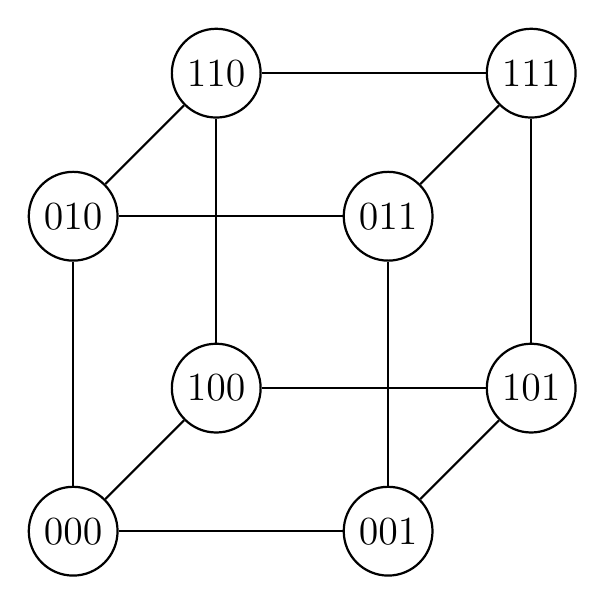
\begin{tikzpicture} [auto, node distance=4cm, every loop/.style={},
                    thick,solmu/.style={circle,draw,font=\sffamily\Large\bfseries}]

\node[solmu] (N000) {$000$};
\node[solmu] (N001) [right of=N000] {$001$};
\node[solmu] (N010) [above of=N000] {$010$};
\node[solmu] (N100) [above right=1cm and 1cm of N000] {$100$};
\node[solmu] (N011) [above of=N001] {$011$};
\node[solmu] (N101) [above right=1cm and 1cm of N001] {$101$};
\node[solmu] (N110) [above right=1cm and 1cm of N010] {$110$};
\node[solmu] (N111) [right of=N110] {$111$};

 \path[every node/.style={font=\sffamily\small}]
    (N000) edge node[left] {} (N001)
    (N000) edge node[left] {} (N010)
    (N000) edge node[left] {} (N100)
    (N001) edge node[left] {} (N011)
    (N001) edge node[left] {} (N101)
    (N010) edge node[left] {} (N110)
    (N010) edge node[left] {} (N011)
    (N100) edge node[left] {} (N101)
    (N100) edge node[left] {} (N110)
    (N110) edge node[left] {} (N111)
    (N101) edge node[left] {} (N111)
    (N011) edge node[left] {} (N111);
\end{tikzpicture}
\end{center}

Tutkitaan hamming-graafien automorfismiryhmää.

Käytetään tässä seuraavia merkintöjä:
\begin{center}
\begin{tabular}{l}
$u + v = (u_1 + v_1, \dots, u_n + v_n) \in \mathbb{Z}_2^n$\\
$1_i \in \mathbb{Z}_2^n$ missä $1_i$:n $i$:s merkki on 1, muut 0.
\end{tabular}
\end{center}
Selvästi $u + u = \hat{0} \forall u \in \mathbb{Z}_2^n$.

Olkoon $G$ hamming-graafi ja $f$ sen automorfismi. Olkoon $u \in G$ ja $v = f(u)$. Koska jokainen $u$:n naapuri kuvatuu $v$:n naapuriksi, yhden merkin muuttaminen $u$:ssa muuttaa yhden merkin $v$:ssä. Automorfismi $f$ ei voi muuttaa samaa $v$:n merkkiä $u$:n naapurustossa, koska muuten $f$ kuvaisi kaksi $u$:n naapuria samaksi alkioksi. Voidaan ajatella, että $f$ permutoi merkkien paikkoja alkion $u$ ympäristössä. 

Olkoon $0 < i, j \leq n, i \neq j$. Alkiot $u + 1_i$ ja $u+ i_j$ ovat $u$:n naapureita, joiden kuvat poikkeavat $v$:stä joillakin indekseillä $i' \neq j'$. Koska $v + 1_{i'} + 1_{j'} = v + 1_{j'} + 1_{i'}$ ja $f(u + 1_i + i_j) = v + 1_{i'} + 1_{j'}$ nähdään että $f(u + 1_i + 1_j) + f(u + 1_i) = f(u + i_j) + f(u)$. Tästä seuraa se, että automorfismin $f$ muodostamat merkkipermutaatiot eivät riipu $u$:n valinnasta. Näin saadaan kuvaus ${\phi: G_S \rightarrow S_n}$, joka kuvaa automorfismit niiden merkkipermutaatioiksi. Kuvaus $\phi$ on selvästi homomorfismi, sillä kahden automorfismin yhdiste yhdistää myös merkkipermutaatiot luonnollisella tavalla.

Tarkastellaan $\phi$:n kerneliä. Symmetrisen ryhmän $S_n$ neutraalialkio on identiteettikuvaus $id$. Automorfismi $f$:n kuva $\phi(f)$ on identiteettikuvaus jos ja vain jos $f(u + 1_i) = f(u) + 1_i \forall u \in G \forall i$. Toisaalta $u = \Sigma 1_k$ jonkin indeksijoukon yli, joten $f(u) = u + f(\bar{0})$. Alkion $\bar{0}$ mahdolliset kuvat määrävät siis $\phi$:n kernelin. Ne muodostavat ryhmän $C_2^n$. Toisaalta ryhmä $S_n$ muodostaa myös $G_S$:n aliryhmän, sillä pelkät merkkipermutaatiot ovat myös automorfismeja. Koska $S_n$ ei muuta merkkejä, ja $C_n^2$ ei permutoi merkkien paikkoja, $S_n \cap C_2^n = \{ id \}$. Koska $C_2^n$ on $\phi$:n kerneli, $C_2^n \trianglelefteq G_S$.

Automorfismiryhmä $G_S$ ei sisällä muita aliryhmiä, sillä mielivaltainen automorfismi voidaan esittää edellä mainittujen automorfismien avulla. Tästä seuraa että $G_S = S_n \rtimes C_2^n$.
\end{example}

\begin{example}
Olkoon $G$ seuraava graafi:

\begin{center}
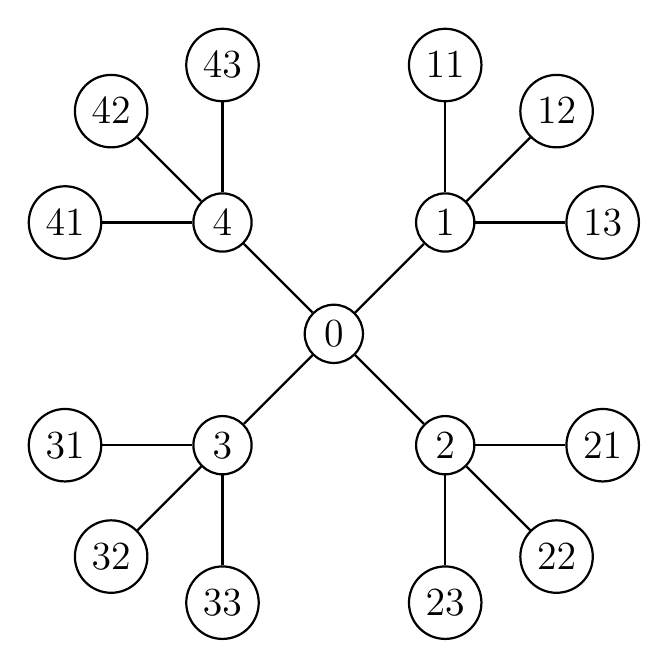
\begin{tikzpicture} [auto, node distance=2cm, every loop/.style={},
                    thick,solmu/.style={circle,draw,font=\sffamily\Large\bfseries}]

\node[solmu] (N0) {$0$};
\node[solmu] (N1) [above right of=N0] {$1$};
\node[solmu] (N2) [below right of =N0] {$2$};
\node[solmu] (N3) [below left of =N0] {$3$};
\node[solmu] (N4) [above left of =N0] {$4$};
\node[solmu] (N11) [above of=N1] {$11$};
\node[solmu] (N12) [above right of =N1] {$12$};
\node[solmu] (N13) [right of =N1] {$13$};
\node[solmu] (N21) [right of=N2] {$21$};
\node[solmu] (N22) [below right of =N2] {$22$};
\node[solmu] (N23) [below of =N2] {$23$};
\node[solmu] (N31) [left of=N3] {$31$};
\node[solmu] (N32) [below left of =N3] {$32$};
\node[solmu] (N33) [below of =N3] {$33$};
\node[solmu] (N41) [left of=N4] {$41$};
\node[solmu] (N42) [above left of =N4] {$42$};
\node[solmu] (N43) [above of =N4] {$43$};

 \path[every node/.style={font=\sffamily\small}]
    (N1) edge node[left] {} (N0)
    (N2) edge node[left] {} (N0)
    (N3) edge node[left] {} (N0)
    (N4) edge node[left] {} (N0)
    (N11) edge node[left] {} (N1)
    (N12) edge node[left] {} (N1)
    (N13) edge node[left] {} (N1)
    (N21) edge node[left] {} (N2)
    (N22) edge node[left] {} (N2)
    (N23) edge node[left] {} (N2)
    (N31) edge node[left] {} (N3)
    (N32) edge node[left] {} (N3)
    (N33) edge node[left] {} (N3)
    (N41) edge node[left] {} (N4)
    (N42) edge node[left] {} (N4)
    (N43) edge node[left] {} (N4);
\end{tikzpicture}
\end{center}

Käytetään alkiosta $0$ termiä runko, alkioista $0 \dots 4$ termiä oksa ja muista alkioista termiä lehti. Helposti nähdään, että graafin $G$:n automorfismit säilyttävät rungon paikallaan, kuvaavat oksat oksiksi ja lehdet lehdiksi. Lisäksi saman oksan lehdet pysyvät yhdessä. Oksat voivat kaikki vaihtaa paikka keskenään, joten kuvaus $\phi$ Olkoon kuvaus $\phi: G_S \rightarrow S_4$ siten että 

\end{example}

\newpage

\section{Fruchtin teoreema}

\begin{teor}
Olkoon $R$ äärellinen ryhmä. Silloin on olemassa äärellinen graafi $G$ siten, että graafin $G$ automorfismiryhmä on isomorfinen $R$:n kanssa.
\begin{proof}
\end{proof}
\end{teor}

\begin{example}
TBW käytetään Fruchtin teoreemaa Klein ryhmään.
\end{example}

\end{document}